\chapter{Cinemática}

\textit{``Si en un instante determinado conociésemos la situación y la velocidad exactas de todas las partículas del universo, 
podríamos deducir por cálculos todo lo pasado y lo futuro de él.''}  \textbf{Laplace}

\section{El movimiento}

\begin{figure}[ht]
 \centering
 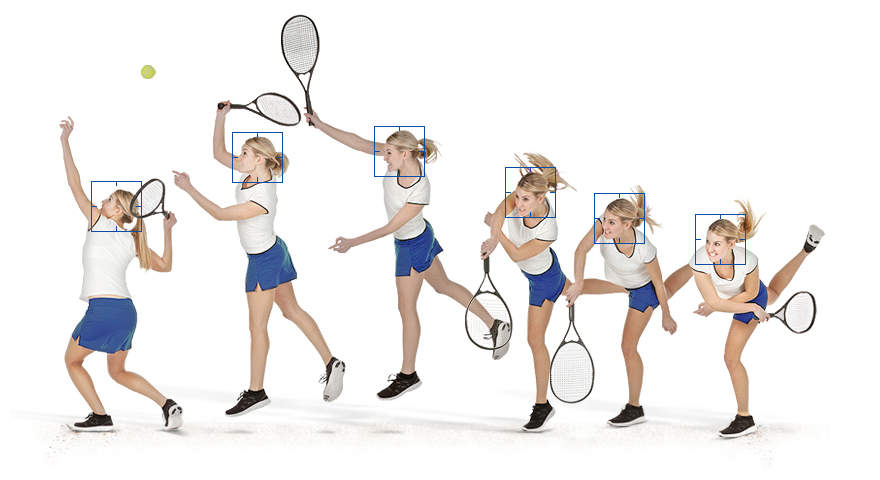
\includegraphics[scale=0.3]{images/movimiento.jpg}
 \caption{Ilustración del movimiento de una tenista.}
 \label{fig:vectorial}
\end{figure}

El estudio de la Física comienza con el fenómeno más fundamental que existe en el Universo el cual es el movimiento. Cada 
componente del Universo está en movimiento, incluso en a temperaturas muy bajas cercanas al cero absoluto el movimiento no cesa, 
y 
es por eso que el movimiento es el fenómeno más fundamental del Universo y el primer apartado a estudiar en Física.\\

La Cinemática es la rama de la Física que estudia a el movimiento sin analizar sus causas, es decir, estudia las magnitudes que 
describen la geometría del movimiento de los cuerpo.\\ 

\begin{figure}[ht]
 \centering
 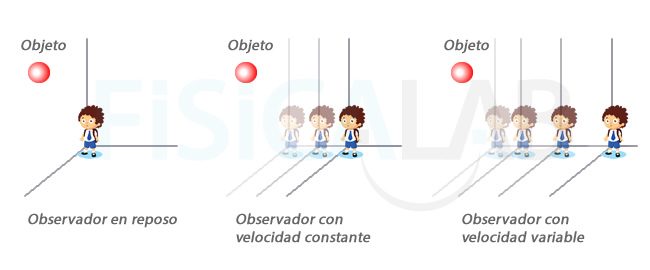
\includegraphics[scale=0.37]{images/sistema_inercial_no_inercial.jpg}
 % sistema_inercial_no_inercial.jpg: 650x270 px, 72dpi, 22.93x9.52 cm, bb=0 0 650 270
 \caption{Ilustración de tres sistemas de referencia diferentes.}
\end{figure}

Para estudiar el fenómeno del movimiento se hace referencia a uno o más observadores que analizan el movimiento y realizan las 
medidas de las magnitudes involucradas en el fenómeno, por ello es necesario plantear un sistema de referencia desde el cual el 
observador u observadores hacen sus medidas, en general el sistema de referencia es el plano cartesiano.\\

Una vez ya ubicado el sistema de referencia lo más natural es observar que el cuerpo o partícula en movimiento tendrá diferentes 
posiciones cuando el tiempo avanza, es por tanto la necesidad de definir lo que se llama vector posición.\\ 

\textbf{Vector posición:} Es el vector que indica la posición del cuerpo respecto a un sistema de referencia. Este vector tiene 
su origen en el origen del sistema de referencia (donde se supone que está un observador) y su extremo donde está el cuerpo o 
partícula de estudio.

\begin{figure}[ht]
 \centering
 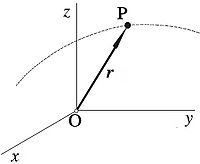
\includegraphics[scale=0.6]{images/posicion.jpg}
 % vector_de_posición.jpg: 200x164 px, 96dpi, 5.29x4.34 cm, bb=0 0 150 123
 \caption{Ilustración del vector posición.}
\end{figure}

Así, si tenemos dos posiciones diferentes del cuerpo o partícula en movimiento se puede definir lo que se llama desplazamiento.\\

\textbf{Desplazamiento:}\\

Se entiende por desplazamiento el vector o segmento recto orientado que une la posición inicial con otra posición posterior en el 
tiempo del cuerpo en movimiento; así, el origen del vector posición es la posición inicial del cuerpo y el extremo del vector 
desplazamiento se halla en la posición final del cuerpo tomada en cuenta. El vector desplazamiento ($\Delta \vec{r}$) resulta de 
hecho la resta del vector posición final ($\vec{r_f}$) con la posición inicial ($\vec{r_o}$).

\begin{equation}
 \Delta \vec{r} = \vec{r_f}-\vec{r_o}
\end{equation}

\begin{figure}[ht]
 \centering
 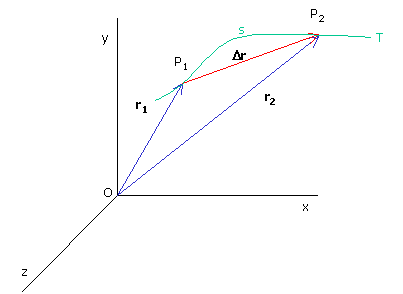
\includegraphics[scale=0.5]{images/cinematica.png}
 % cinematica.png: 0x0 px, 300dpi, 0.00x0.00 cm, bb=
 \caption{Ilustración del vector desplazamiento.}
\end{figure}

\textbf{Trayectoria:}\\

La trayectoria es el camino por el cual el cuerpo en movimiento\footnote{Muchas veces a un cuerpo en movimiento también se le 
dice móvil en Física.} se mueve.

\begin{figure}[ht]
 \centering
 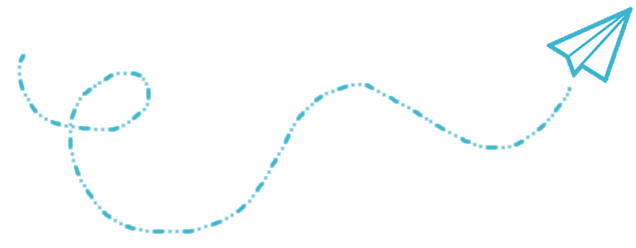
\includegraphics[scale=0.4]{images/trayectoria.png}
 % cinematica.png: 0x0 px, 300dpi, 0.00x0.00 cm, bb=
 \caption{Ilustración de la trayectoria de un avión de papel.}
\end{figure}

\textbf{Distancia:}\\

En Física, la distancia es la longitud total recorrida por un objeto móvil en su trayectoria. Como tal, es una magnitud escalar, 
y, por lo tanto, es expresada en unidades de longitud (En el SI en metros).\\

\textbf{Velocidad:}\\

La velocidad ($\vec{v}$) es una cantidad vectorial muy usada en Física que mide el ritmo de cambio de la distancia recorrida por 
un móvil con respecto al tiempo, y en este vector brinda la idea de cuan rápido o tan despacio se mueve un cuerpo. El módulo de 
la velocidad se llama rápidez o celeridad, generalemente se simboliza simplemente como $v$ y se la mide en el SI en $m/s$. 

\begin{equation}
 v = \frac{\text{distancia recorrida}}{\text{tiempo necesario para el movimiento}} \quad [m/s]
\end{equation}

\begin{equation}
 \vec{v} = \frac{\Delta \vec{r}}{\Delta t}
\end{equation}

Una de las principales características del vector velocidad es que siempre es tangente a la trayectoria que sigue el móvil.

\begin{figure}[ht]
 \centering
 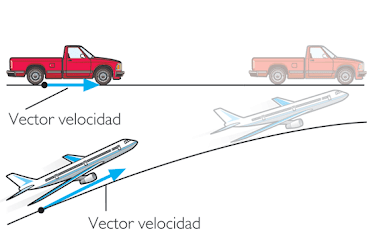
\includegraphics[scale=0.4]{images/vectorvelocidad.png}
 % cinematica.png: 0x0 px, 300dpi, 0.00x0.00 cm, bb=
 \caption{Ilustración del vector velocidad.}
\end{figure}

\textbf{Velocidad instantánea:}\\

 Es la que tiene el cuerpo en un instante específico, en un punto determinado de su trayectoria. Se define la velocidad 
instantánea o simplemente velocidad como el límite de la velocidad media cuando el intervalo de tiempo considerado tiende a 0. 
Esta velocidad es la que marca el velocímetro dentro de un auto por ejemplo.

 \begin{equation}
 \vec{v}=\lim_{\Delta t \to 0}\frac{\Delta \vec{r}}{\Delta t}\quad [m/s]
 \end{equation}

Una vez comprendido estos conceptos fundamentales del movimiento es tiempo de analizar el movimiento más simple que existe: 
\textit{El movimiento rectilíneo}.

\subsection*{Problemas}

\begin{enumerate}
 \item ¿Cuál es el desplazamiento realizado por un móvil que partió desde la posición $\vec{r_0} = 20 km;N34^\circ O$ hacia la 
posición $\vec{r_f} = 30 km; S45^\circ E$? 

\item Si el desplazamiento realizado por el móvil del problema anterior fue realizado en un tiempo promedio de 4 minutos,¿cuál es 
la velocidad promedio desarrollada por dicho móvil?

\end{enumerate}
